%%%% Dokumentklassen %%%%

\documentclass[a4paper,11pt,fleqn,dvipsnames,oneside,openany]{memoir} 	% Openright åbner kapitler på højresider (openany begge)



%%%% PACKAGES %%%%

%% Oversættelse og tegnsætning %%
\usepackage[utf8]{inputenc}					% Input-indkodning af tegnsæt (UTF8)
\usepackage[danish]{babel}					% Dokumentets sprog
\usepackage[T1]{fontenc}					    % Output-indkodning af tegnsæt (T1)
\usepackage{ragged2e,anyfontsize}			% Justering af elementer
\usepackage{fixltx2e}						% Retter forskellige fejl i LaTeX-kernen

\usepackage{lastpage}						% Total antal sider opdateres automatisk ved \pageref{LastPage}
																			
%% Figurer og tabeller (floats) %%
\usepackage{graphicx} 						% Håndtering af eksterne billeder (JPG, PNG, EPS, PDF)
\usepackage{multicol}         	            	% Muliggør output i spalter
\usepackage{rotating}						% Rotation af tekst med \begin{sideways}...\end{sideways}
\usepackage{xcolor}							% Definer farver med \definecolor. Se mere: http://en.wikibooks.org/wiki/LaTeX/Colors
\usepackage{flafter}						% Sørger for at floats ikke optræder i teksten før deres reference
\let\newfloat\relax 						% Justering mellem float-pakken og memoir
\usepackage{float}							% Muliggør eksakt placering af floats, f.eks. \begin{figure}[H]

%% Matematik mm. %%
\usepackage{amsmath,amssymb,stmaryrd} 		% Avancerede matematik-udvidelser
\usepackage{mathtools}						% Andre matematik- og tegnudvidelser
\usepackage{textcomp}                 		% Symbol-udvidelser (fx promille-tegn med \textperthousand)
\usepackage{rsphrase}						% Kemi-pakke til RS-saetninger, fx \rsphrase{R1}
\usepackage[version=3]{mhchem} 				% Kemi-pakke til flot og let notation af formler, f.eks. \ce{Fe2O3}
\usepackage{siunitx}						% Flot og konsistent præsentation af tal og enheder med \si{enhed} og \SI{tal}{enhed}
\sisetup{output-decimal-marker = {,}}		% Opsætning af \SI (DE for komma som decimalseparator) 

%% Referencer og kilder %%
\usepackage[danish]{varioref}				% Muliggør bl.a. krydshenvisninger med sidetal (\vref)
%\usepackage{natbib}							% Udvidelse med naturvidenskabelige citationsmodeller

\usepackage[backend=bibtex, maxnames=1, url=false, style=science, natbib=true]{biblatex}
\addbibresource{Bibliografi/Ref.bib}


\usepackage{xr}							    % Referencer til eksternt dokument med \externaldocument{<NAVN>}

%% Misc. %%
\usepackage{listings}						% Placer kildekode i dokumentet med \begin{lstlisting}...\end{lstlisting}
\usepackage{lipsum}							% Dummy text \lipsum[..]
\usepackage[shortlabels]{enumitem}			% Muliggør enkelt konfiguration af lister
\usepackage{pdfpages}						% Gør det muligt at inkludere pdf-dokumenter med kommandoen \includepdf[pages={x-y}]{fil.pdf}	
\pdfoptionpdfminorversion=6					% Muliggør inkludering af pdf-dokumenter, af version 1.6 og højere
\pretolerance=2500 							% Justering af afstand mellem ord (højt tal, mindre orddeling og mere luft mellem ord)


%%%% CUSTOM SETTINGS %%%%

%% Marginer %%
\setlrmarginsandblock{2.5cm}{2.5cm}{*}		% \setlrmarginsandblock{Indbinding}{Kant}{Ratio}
\setulmarginsandblock{2.5cm}{3.0cm}{*}		% \setulmarginsandblock{Top}{Bund}{Ratio}
\checkandfixthelayout 						% Oversætter værdier til brug for andre pakker

%% Afsnitsformatering %%
\setlength{\parindent}{0mm}           		% Størrelse af indryk
\setlength{\parskip}{3mm}          			% Afstand mellem afsnit ved brug af double Enter
\linespread{1,1}							% Linjeafstand

%% Indholdsfortegnelse %%
\setsecnumdepth{subsection}		 			% Dybden af nummererede overskrifter (part/chapter/section/subsection)
\maxsecnumdepth{subsection}					% Dokumentklassens grænse for nummereringsdybde
\settocdepth{subsection} 					% Dybden af indholdsfortegnelsen
		
%% Opsætning af listings %%
\definecolor{commentGreen}{RGB}{34,139,24}
\definecolor{stringPurple}{RGB}{208,76,239}

\lstset{language=Matlab,					    % Sprog
	basicstyle=\ttfamily\scriptsize,		    % Opsætning af teksten
	keywords={for,if,while,else,elseif,		% Nøgleord at fremhæve
			  end,break,return,case,
			  switch,function},
	keywordstyle=\color{blue},				% Opsætning af nøgleord
	commentstyle=\color{commentGreen},		% Opsætning af kommentarer
	stringstyle=\color{stringPurple},		% Opsætning af strenge
	showstringspaces=false,					% Mellemrum i strenge enten vist eller blanke
	numbers=left, numberstyle=\tiny,		    % Linjenumre
	extendedchars=true, 					    % Tillader specielle karakterer
	columns=flexible,						% Kolonnejustering
	breaklines, breakatwhitespace=true,		% Bryd lange linjer
}

%% Navngivning %%
\addto\captionsdanish{
	\renewcommand\appendixname{Appendiks}
	\renewcommand\contentsname{Indholdsfortegnelse}	
	\renewcommand\appendixpagename{Appendiks}
	\renewcommand\appendixtocname{Appendiks}
	\renewcommand\cftchaptername{\chaptername~}		% Skriver "Kapitel" foran kapitlerne i indholdsfortegnelsen
	\renewcommand\cftappendixname{\appendixname~}	% Skriver "Appendiks" foran appendiks i indholdsfortegnelsen
}

%% Kapiteludssende %%
\definecolor{numbercolor}{gray}{0.7}		            % Definerer en farve til brug til kapiteludseende
\newif\ifchapternonum

\makechapterstyle{jenor}{					        % Definerer kapiteludseende frem til ...
  \renewcommand\beforechapskip{0pt}
  \renewcommand\printchaptername{}
  \renewcommand\printchapternum{}
  \renewcommand\printchapternonum{\chapternonumtrue}
  \renewcommand\chaptitlefont{\fontfamily{pbk}\fontseries{db}\fontshape{n}\fontsize{25}{35}\selectfont\raggedleft}
  \renewcommand\chapnumfont{\fontfamily{pbk}\fontseries{m}\fontshape{n}\fontsize{1in}{0in}\selectfont\color{numbercolor}}
  \renewcommand\printchaptertitle[1]{%
    \noindent
    \ifchapternonum
    \begin{tabularx}{\textwidth}{X}
    {\let\\\newline\chaptitlefont ##1\par} 
    \end{tabularx}
    \par\vskip-2.5mm\hrule
    \else
    \begin{tabularx}{\textwidth}{Xl}
    {\parbox[b]{\linewidth}{\chaptitlefont ##1}} & \raisebox{-15pt}{\chapnumfont \thechapter}
    \end{tabularx}
    \par\vskip2mm\hrule
    \fi
  }
}											        % ... her

\chapterstyle{jenor}						        % Valg af kapiteludseende - Google 'memoir chapter styles' for alternativer

%% Sidehoved %%

\makepagestyle{AAU}							        % Definerer sidehoved og sidefod udseende frem til ...
\makepsmarks{AAU}{%
	\createmark{chapter}{left}{shownumber}{}{. \ }
	\createmark{section}{right}{shownumber}{}{. \ }
	\createplainmark{toc}{both}{\contentsname}
	\createplainmark{lof}{both}{\listfigurename}
	\createplainmark{lot}{both}{\listtablename}
	\createplainmark{bib}{both}{\bibname}
	\createplainmark{index}{both}{\indexname}
	\createplainmark{glossary}{both}{\glossaryname}
}
\nouppercaseheads									% Ingen Caps ønskes

\makeevenhead{AAU}{\small ST3PRJ3 Gruppe 2}{}{\leftmark}	% Definerer lige siders sidehoved (\makeevenhead{Navn}{Venstre}{Center}{Hoejre})
\makeoddhead{AAU}{\rightmark}{}{\small ASE}		            % Definerer ulige siders sidehoved (\makeoddhead{Navn}{Venstre}{Center}{Højre})
\makeevenfoot{AAU}{\small \thepage}{}{}						% Definerer lige siders sidefod (\makeevenfoot{Navn}{Venstre}{Center}{Højre})
\makeoddfoot{AAU}{}{}{\small \thepage}						% Definerer ulige siders sidefod (\makeoddfoot{Navn}{Venstre}{Center}{Højre})

\copypagestyle{AAUchap}{AAU}							% Sidehoved for kapitelsider defineres som standardsider, men med blank sidehoved
\makeoddhead{AAUchap}{}{}{}
\makeevenhead{AAUchap}{}{}{}
\makeheadrule{AAUchap}{\textwidth}{0pt}
\aliaspagestyle{chapter}{AAUchap}					% Den ny style vælges til at gælde for chapters
													% ... her
															
\pagestyle{AAU}										% Valg af sidehoved og sidefod


%%%% CUSTOM COMMANDS %%%%

%% Billede hack %%
\newcommand{\figur}[4]{
		\begin{figure}[H] \centering
			\includegraphics[width=#1\textwidth]{billeder/#2}
			\caption{#3}\label{#4}
		\end{figure} 
}

%% Specielle tegn %%
\newcommand{\decC}{^{\circ}\text{C}}
\newcommand{\dec}{^{\circ}}
\newcommand{\m}{\cdot}


%%%% ORDDELING %%%%

\hyphenation{}


%%%% Tilføjelser af min preample %%%%

% Booktabs:
% The booktabs package is needed for better looking tables. 
\usepackage{booktabs}

% Caption:
% For better looking captions. See caption documentation on how to change the format of the captions.
\usepackage[hang, font={small, it}]{caption}

% Hyperref:
% This package makes all references within your document clickable. By default, these references will become boxed and colored. This is turned back to normal with the \hypersetup command below.
\usepackage{hyperref}
	\hypersetup{colorlinks=false,pdfborder=0 0 0}

% Cleveref:
% This package automatically detects the type of reference (equation, table, etc.) when the \cref{} command is used. It then adds a word in front of the reference, i.e. Fig. in front of a reference to a figure. With the \crefname{}{}{} command, these words may be changed.
\usepackage{cleveref}
	\crefname{equation}{formel}{formler}
	\crefname{figure}{figur}{figurer}	
	\crefname{table}{tabel}{tabeller}

% Mine tilføjelser:
\usepackage{units}                        %% Bruges til at gøre fx 1/2 samlet med: \nicefrac{1}{2}.
\usepackage{tabu, longtable}              %% Bruges til tabeller.
\setlength{\tabulinesep}{1.5ex}           %% Definerer linjeafstand i tabeller.
\usepackage{enumerate}                    %% Bruges til lister.
\usepackage{tabto}                        %% Giver mulighed for TAB med fx \tabto{3em}.
\usepackage[hyphenbreaks]{breakurl}       %% Bruges til websiders url'er.
\renewcommand{\UrlFont}{                  %% Definerer url-font.
\small\ttfamily}                          %
%\bibliographystyle{unsrt}                 %% Definere bibliografien. Ses til sidst i dokumentet i kapitlet Litteratur.
\usepackage{amssymb} 
\usepackage{pifont}
%\newcommand{\xmark{\ding{55}}			 % Opretter et unchecked mark
\usepackage{url}

\usepackage{pifont}
\usepackage{nccmath}						% Bruges til centering af equations (\begin{ceqn})



\usepackage{url}
\usepackage{hyperref}
%\usepackage{natbib}
%\bibliographystyle{plainnat}
%\usepackage{biblatex}

\raggedbottom

%\externaldocument[D-]{Dokumentation}

\begin{document}

	
\frontmatter						% Nummereres med romerske tal.
\let\cleardoublepage\clearpage
\begin{titlingpage}
\begin{center}
~ \\[3cm]


\includegraphics[width=0.6\textwidth]{figurer/ASE}~\\[1cm]

\textsc{\LARGE Aarhus School of Engineering}\\[1.5cm]

\textsc{\Large Sundhedsteknologi}\\
\textsc{\Large Medicinsk Teknologi Vurdering }\\[0.5cm]

\noindent\makebox[\linewidth]{\rule{\textwidth}{0.4pt}}\\
[0.5cm]{\Huge Ultralyds Robotarm}
\noindent\makebox[\linewidth]{\rule{\textwidth}{0.4pt}}

\end{center}

Anne Bundgaard Hoelgaard\tab(201404492) \newline
Ditte Heebøll Callesen\tab(201408392) \newline
Freja Ramsing Munk\tab(2014) \newline
Ida Mark Skovbjerg\tab(2014) \newline	
Mette Østergård Knudsen\tab(2014) \newline 
Nina Brkovic\tab(2014) \newline 


\textit{Vejledere:} \newline
Lene Hause\\
Samuel Alberg Thrysøe
Aarhus Universitet

\vfill

\begin{center}
{\large 16. december 2015}
\end{center}

\end{titlingpage}
\chapter{Abstract} 
\subsubsection{Introduction}
Sonographers who work with ultrasonic examination of pregnant women are at risk of getting work-related disorder due to poor work postures. It is often necessary to press the ultrasonic probe against the stomach, while the probe is being held at arm’s length. An Ultrasonic Robotic Arm will reduce the amount of poor work postures. The Robotic Arm where the ultrasonic probe is attached will be controlled by the sonographer with a joystick. The sonographer thereby avoids the previously mentioned physical challenges and potential discomforts. 

\subsubsection{Methods}
The purpose of this report has been to study which consequences the implementation of the Ultrasonic Robotic Arm can have with focus on four perspectives: Technology, Organization, Patient, and Economics. 
Information which can be used in all perspectives has been obtained through interviews with departments for ultrasonic examinations of pregnant women in the Regional Hospital of Horsens and the Regional Hospital of Viborg. Specific methods has been used for each perspective.

\subsubsection{Discussion}
This report is based on a summary of interviews, scientific articles, and assumptions. This is partly because the Ultrasonic Robotic Arm is not fully developed, which causes an insecurity which could have been reduced throughout other researches. 
The Ultrasonic Robotic Arm can be used as equipment for telemedicine in the future. This will require an attachment of a camera and a microphone to the system. There will be no direct changes to the Ultrasonic Robotic Arm. The sonographer does not need to be in the same room as the pregnant woman during the ultrasonic examination. 

\subsubsection{Conclusion} 
The Ultrasonic Robotic Arm will be able to reduce the amount of work-related disorder and poor work postures for sonographers during ultrasonic examination of pregnant women. The sonographers will be able to perform ultrasonic examinations 37 hours a week and stay in the job for a greater amount of years. The Robotic Arm will not lead to changes for the patient with regard to the quality and the result of the ultrasonic examination. 
The Ultrasonic Robotic Arm has a technological restriction, which means it can be used for 70-80\% of the ultrasonic examinations of pregnant women. The remaining 20-30\% of the ultrasonic examinations must be performed manually. From an economic perspective savings in wage costs will not cover the annual depreciation provision on the purchase of the Ultrasonic Robotic Arm.



\chapter{Resumé}

%\begin{figure}[h!]\centering
%	\includegraphics[width = 0.4\textwidth]{Filnavn}
%	\caption{Billede 1}
%	\label{billede1}
%\end{figure}
%\chapter{Forord}
Denne mini-MTV er udarbejdet på 4. semester på Sundhedsteknologi, Aarhus Universitet Ingeniørhøjskolen (IHA), under vejledning af Lene Häuser Petersen og Samuel Alberg Thrysøe. Projektet tager sit udgangspunkt i undervisningen på IHA, og udspringer fra kurset Medicinsk Teknologi Vurdering. 


I forbindelse med udformningen af denne mini Medicinsk Teknologi Vurdering vil vi gerne takke følgende personer og afdelinger, for deres venlighed og hjælp:


Tak til Tina Arnbjørn fra Hospitalsenheden Horsens, Kvindeafdelingen, Svangre- og Ultralydsambulatorium for at stille op til interview, og tak til afdelingen for demonstrering af ultralydsscanninger. 


Tak til Karen Marie Goul fra Regionshospital Midt Viborg, Kvindesygdomme og Fødsler for at stille op til interview. Samt et tak til afdelingen for demonstrationer af ultralydsscanninger. 


Endvidere skal der lyde en stor tak til Søren Pallesen for idegrundlag, hans viden omkring Ultralyds Robotarmen, samt inspiration til litteratursøgning. 


\chapter{Forkortelser og formler}

\section{Forkortelser}
\begin{longtabu} to \linewidth{@{}l X[j]@{}}
    Ord &    Forklaring\\
    \toprule\ \\
    Robotarm & Ultralyds robotarm udviklet af Robotic Ultrasound ApS \\
    MTV & Medicinsk Teknologi Vurdering \\
  	RMV & Regionshospital Midt Viborg, Kvindesygdomme og Fødsler \\
  	HEH & Hospitalsenheden Horsens, Kvindeafdelingen, Svangre- og Ultralydsambulatorium \\
  	BMI & Body Mass Index \\
  	Bilag 12, 28.04.2016 & Se bilag 12 under dato 28.04.2016
   
\label{forkort}
\end{longtabu}

\section{Formler} \label{Formler}
Annunitetsmetoden: \\
Viser den gennemsnitlige årlige værdi af en investering. Baseret på den forventede levetid og en pålagt årlig rente.
\begin{equation}
\left( \dfrac{(1+\text{rente})^{\text{forventet levetid}}\cdot \text{rente}}{(1+\text{rente})^{\text{forventet levetid}}-1}\right)\cdot \text{udstyrspris} = \text{gennemsnitlige årlige værdi}
\end{equation}
%\chapter{Formler}


%\cleardoublepage	
	
\tableofcontents*                   % Indsætter en indholdsfortegnelse før Indledning.
%\addcontentsline{toc}{List of Figures}	%Tilføjer liste af figurer i indholdsfortegnelsen. 

\mainmatter                         % Her findes de nummererede kapitler modsat \frontmatter og \backmatter. Nummereres med arabiske tal.

\chapter{Indledning} 
Ved ultralydsscanning af gravide er arbejdsgener (og -skader) hos sonograferne et kendt problem. For at udføre scanningerne holder sonograferne proben i akavede stillinger, der udsætter deres skulder, arm og håndled for store belastninger \textbf{(reference)}. Hvilket blot forøges når et pres på mellem 3 og 11 kg. kræves for at få et klart ultralydsbillede \textbf{(reference til Søren)}. Disse stillinger øger risikoen for at få arbejdsskader. Grundet sonografernes belastende arbejdsstillinger er der fra Dansk Føtalmedicinsk Selskab udstukket guidelines angående det maksimale antal timer, en sonograf anbefales at foretage scanninger i løbet af en uge. Disse guidelines er på 28 timer om ugen \textbf{(reference)}. Dette gør at der skal flere sonografer til for at kunne scanne det stigende antal gravide i Danmark.\cite{Foedsler}. \\
Samtidig er Danmark inde i en udvikling, der gør at antallet af overvægtige stiger \cite{Overvaegt}. Dette gør at sonograferne skal presse med en større kraft for at få billeder af tilsvarende kvalitet frem. 

Gennem en årrække er der lavet en række forskningsstudier og forsøg med robotarm til ultralydsscanning af hjertet \textbf{(reference – artikel 8)}. Dette er med til at underbygge, at problemstillingen er kendt, men samtidig også at den optimale metode endnu ikke er fundet. Yderligere findes der flere forskningsstudier der drejer sig om udviklingen af robotter til lignende opgaver \textbf{(reference)}. Dette viser, at det er et område der investeres penge i og hvor der er en tro på at der er en fremtid i. 

Denne udvikling har ført til, at firmaet Robotic Ultrasound ApS er i færd med at udvikle en Ultralyds Robotarm, der formodentlig kan afhjælpe problemet. Denne robotarm styres via et joystick, således at sonograferne kan undgå at være i de akavede arbejdsstillinger, men i stedet kan styre robotten til de ønskede stillinger. 

%Problemstillingen i denne form er et område der ikke tidligere er afdækket. Men tidligere forskning i forhold til ultralydsscanning med robot gør at der findes tilstrækkelig videnskabelig dokumentation til at bygge mini-MTV’en op omkring. 

\section{Formål}
Formålet med denne mini-MTV er derfor at vurderer om Ultralyds Robotarmen kan implementeres som en teknologisk aflastnings løsning for sonografer i deres arbejde med scanning af gravide. Det ønskes at klarlægge fordele og ulemper ved både de eksisterende arbejdsforhold, og forholdene ved implementering af Ultralyds Robotarmen, samt hvilke forskelle robotarmen vil medføre for sonografer og gravide.

Yderligere forventes det, at rapportens resultater vil blive efterspurgt forud for en beslutningstagning når robotarmen er færdigudvikler og produceret. Dermed er formålet med mini-MTV’en også at bidrage til beslutningsgrundlaget for den enkelte sygehusafdeling, om Ultralyds Robotarmen skal implementeres, og i så fald hvilke aspekter der skal tages højde for og medtages i en vurdering. \textbf{Reference til metodehåndbog??}

\section{Projektafgrænsning}
Projektet afgrænses til en vurdering af, hvorvidt det kan betale sig at gøre brug af en Ultralyds Robotarm ved scanning af gravide i forhold til det udstyr der benyttes på afdelingerne i dag. Det primære fokus i projektet er problemstillingen om, at et stort antal sonografer oplever arbejdsskader og -gener ved scannings arbejdet \textbf{(reference)}. 

Ultralyds robotarmen åbner også for muligheden om, at bruge denne som en telemedicinsk løsning, hvor selve sonografen der foretager scanningen er placeret på et andet sygehus. Dette aspekt er det fravalgt at vurdere på i denne mini-MTV. 

Opgaven er afgrænset til at en 25 siders rapport, hvor det skriftlige omfang på en typisk dansk MTV ligger på over 100 sider. Dette gør, at det er en mini-MTV der udarbejdes. I en mini-MTV vurderes problemstillingen på de fire parametre: \textit{organisation, patient, teknologi og økonomi.} 

Den korte tidshorisont til udarbejdelsen af denne mini-MTV har været en afgørende faktor for, at det er valgt at begrænse projektet til at bygge på interview med to relevante danske sygehus afdelinger, samt en litteratursøgning på problemstillingen. Normalt er udarbejdelsen af en MTV en lang proces, da det kræver stort researcharbejde. Interview er afholdt med ”Kvindeafdelingen, Svangre- og Ultralydsambulatorium” på Hospitalsenheden Horsens (HEH) og afdelingen ”Kvindesygdomme og Fødsler” på Regionshospitalet Viborg (RMV).

\section{Projektorganisation}
Projektet er blevet udarbejdet som semesterprojekt af seks sundhedsteknologistuderende på 4. semester ved Ingeniørhøjskolen Aarhus Universitet. De studerende har været i en projektgruppe. \\
Hovedforfattere til de enkelte kapitlerne er:
\begin{itemize}
\item \textit{Organisation: }Anne Hoelgaard, Ida Skovbjerg og Nina Brkovic
\item \textit{Patient: }Ditte Callesen, Nina Brkovic og Freja Munk
\item \textit{Teknologi: }Ida Skovbjerg, Ditte Callesen og Mette Knudsen
\item \textit{Økonomi: }Anne Hoelgaard, Freja Munk og Mette Knudsen
\end{itemize}

\label{version_Systemark}
%\end{longtabu}
\chapter{Metoder}
Afsnittet indeholder en beskrivelse af hvilke metoder, der er blevet anvendt til udarbejdelse af denne mini-MTV i forhold til de fire MTV aspekter: Teknologi, Patient, Organisation og Økonomi.

Overordnet set er der blevet gennemført en litteratursøgning og -vurdering på baggrund af en i forvejen opstillet protokol (Bilag xx). Protokollen er udarbejdet ud fra specifikke søgestrategier, hvor der er søgt på både engelsk og dansk. De specifikke søgeord er medtaget som dokumentation. Der er søgt i følgende databaser: Embase, PubMed, Google Scholar, Cochrane og Engineering Village. \\
De fremsøgte artikler er blevet sorteret ud fra inklusions- og eksklusionskriterier. Artikler, som omhandlede specifikt telemedicin er blevet ekskluderet, da indholdet ikke er relevant for problemstillingen. Artikler omhandlende scanning af gravide, scanning af hjertet, robotarm og arbejdsskader hos sonografer er inkluderet i mini-MTV’en.\\
Udover ovenstående litteratur er der, efter behov søgt efter ikke videnskabelig litteratur for at opnå en forståelse for opbygningen af sonograf uddannelse, ultralydsscanning og andre løse emner for at komme ind i problemstillingen. 

\section{Teknologi}
Dataindsamling til Teknologiafsnittet er sket via antagelser fra CEO Søren Pallesen, Robotic Ultrasound ApS og produktspecifikationer fra Universal Robots, samt information fra interview og samtale med sonografer på HEH og RVM. Afsnittet belyser Ultralyds Robotarmens anvendelsesområder, specifikationer samt sikkerhedsindstillinger.
\section{Patient}
Patientafsnittet bygger på data fra interview og samtale med sonografer på HEH, samt viden fra etik undervisning. Derudover er de fem patientperspektiver – sociale, økonomiske, etiske, individuelle og kommunikative forhold – blevet benyttet til at belyse den pågældende teknologi og de faktorer, der har betydning for patientens hverdagsliv.\\ 
Den etiske vurdering tager udgangspunkt i problemstillinger, der påvirker gravide og sonografer. Disse problemstillinger omhandler de professionsetiske principper, som den etiske vurdering er baseret på.
\section{Organisation}
Dataindsamling til Organisationsafsnittet er sket via direkte kontakt til kilder gennem interviews i både HEH og RMV. Afsnittet belyser betydningen af implementeringen af den nye teknologi for afdelingen som organisation samt mulige ændringer for personalet. Derudover er Leavitts organisationsmodel blevet benyttet til at beskrive de fire organisatoriske hovedelementer.

\section{Økonomi}
Den økonomiske dataindsamling er primært sket på baggrund af direkte kontakt til kilder via telefon eller mailkorrespondance. Derefter er dokumenter og andre skriftlige kilder afsøgt, typisk ved at holde dem op mod mundtlige kilder. Vurderingen er udarbejdet med udgangspunkt i Omkostningsminimeringsanalyse (CMA). De økonomiske beregninger indeholder flere af projektgruppens antagelser, hvor det ikke har været muligt at finde kilder med tilstrækkelig økonomisk evidens. 
%\chapter{De fire MTV-elementer}


\chapter{Organisation} \label{Organisation}
Dette afsnit vil give et indblik i strukturen og opbygningen af Kvindeafdelingen, Svangre- og ultralydsambulatorium på Hospitalsenheden Horsens (HEH) og afdeling Kvindesygdomme og Fødsler på Regionshospitalet Midt Viborg (RMV). Afsnittet vil belyse, hvilken betydning, implementeringen af en Ultralyds Robotarm vil have for afdelingerne som organisation, samt de ændringer det medfører i arbejdsgangen for personalet. \\
Informationer, som er indhentet fra HEH og RMV, vil blive sammenholdt med videnskabelige artikler i et forsøg på at finde en større sammenhæng i problemstillingen omkring arbejdsgener ved ultralydsscanning af gravide. 

Det er valgt at benytte Leavitts organisationsmodel, se figur \ref{DiamantModel}, som analysemetode. Denne model er en diamantmodel, der arbejder med fire organisatoriske hovedelementer, som relaterer til hinanden. Hvert hovedelement vil blive belyst i hvert sit underafsnit \cite{Leavitt} \cite{diamantmodel}. 

\begin{figure}[h!]\centering
	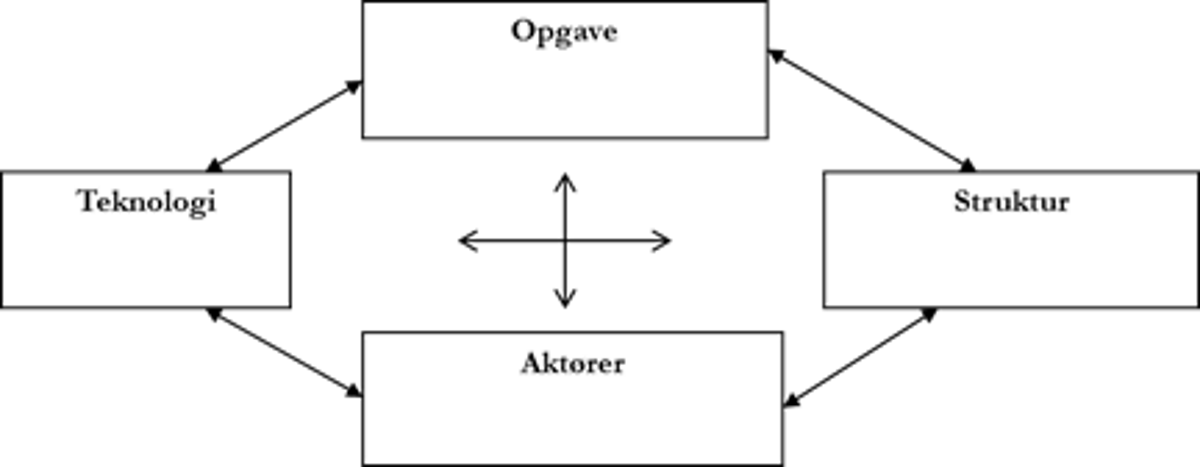
\includegraphics[width = 0.7\textwidth]{Figurer/LeavittModel}
	\caption{Leavitts organisationsmodel, viser hvordan struktur, aktører, opgaver og teknologi indbyrdes relaterer til hinanden \cite{diamantmodel}.}
	\label{DiamantModel}
\end{figure}

Da analysen bygger på dataindsamling fra to kliniske afdelinger, HEH og RMV, vil dens generaliserbarhed potentielt være begrænset. Resultatet heraf kan derfor ikke nødvendigvis anvendes på lignende hospitalsafdelinger i Danmark. 

Dataindsamlingen til analysen er indhentet gennem interview med afdelingssygeplejerske Tina Arnbjørn og tre sonografer fra HEH, samt interview med afdelingssygeplejerske Karen Marie Goul og en sonograf fra RMV.
Til at underbygge problemstillingen omkring arbejdsgener suppleres der med videnskabelige artikler.

\section{HEH}
HEH er bemandet af en afdelingssygeplejerske, fem sonografer samt et ukendt antal læger. Antallet af læger er ikke relevant for denne analyse, da der udelukkende fokuseres på sonografernes arbejdsgange.
Afdelingen har udstyr til fire stuer, hvoraf tre stuer bemandes af sonografer. Der foretages 30-40 scanninger om dagen på afdelingen, og hver scanning tager i gennemsnit 35 minutter. 
Ovenstående information er blevet opsamlet under interview med afdelingssygeplejerske Tina Arnbjørn på HEH, se Bilag 4.

\section{RMV}
Bemanding på RMV består af en afdelingssygeplejerske, ni sonografer og et ukendt antal læger. Afdelingen har ultralydsscanningsudstyr til fem stuer til gravide, hvoraf tre stuer er i drift dagligt og bemandes af sonografer. Dagligt foretages der 25-30 scanninger på afdelingen. En scanning tager i gennemsnittet 30 minutter.
Informationerne for RMV er opnået igennem interview med en sonograf fra afdelingen og afdelingssygeplejerske Karen Marie Goul, se Bilag 5.

\section{Leavitts organisationsmodel}
Det er valgt at sammenskrive de indsamlede data fra HEH og RMV, da afdelingerne er sammenlignelige. Leavitts organisationsmodel vil klarlægge afdelingers organisation og struktur. Derudover vil modellen belyse, hvordan organisationsstrukturen, opgaver og organisationens ansatte bliver påvirket af implementeringen af den nye teknologi \cite{Leavitt} \cite{diamantmodel}. 


\subsection{Opgaver}
Opgaverne som afdelingerne varetager på nuværende tidspunkt vil ikke ændre sig ved implementering af robotarmen, da behovet for scanninger af gravide er uændret. Opgaverne består af nakkefoldsscanning i 11.-13. uge, misdannelsesscanning i 19.-22. uge, vægtscanninger samt diverse kontrolscanninger under graviditeten \cite{graviditet}.

\subsection{Teknologi}
Ved implementering af en ny teknologi, som Ultralyds Robotarmen, sættes der krav til aktørernes faglige kundskaber og erfaringer i brugen af teknologien. Dette er gældende for samtlige sonografer, der skal benytte robotarmen. Der skal derfor være en indkørselsperiode af teknologien førend, den vil være i fuld brug, og før alt personale har kompetencerne til brugen af robotarmen. \\
Det vurderes, at de eksisterende stuer på HEH og RMV er tilstrækkelig store til, at teknologien vil kunne implementeres uden yderligere ændringer. På RMV kan det dog blive nødvendigt at flytte patientskærmen, da robotarmsstativet, se kapitel \ref{Teknologi}, muligvis vil komme til at dække for den gravides udsyn til skærmen.  

\subsection{Aktører} \label{aktoerer_organisation}
Muskel- eller skeletbesvær forårsaget eller forværret af de arbejdsopgaver, som udføres på arbejdspladsen er af typen work-related musculoskeletal disorders (WRMSD). De fremkommer ved gentagne belastninger, kraftkrævende eller akavede bevægelser. I 2008 oplevede op til 90\% af sonograferne smerter under udførelsen af scanninger. Disse smerter kan blive en økonomisk og \textbf{personlig udgift - hvordan personlig?} for sonograferne \cite{31}\cite{30}\citep{24}\cite{36}.\\
På både HEH og RMV underbygger udtalelser fra sonograferne billedet af, at mange af dem oplever smerter under scanninger. 
Her er den udbredte mening, at arbejdet er belastende, og der er usikkerhed om, hvor længe de kan blive i stillingen. Det belastende arbejde, samt den stigende tendens for kvinders BMI, bidrager til denne usikkerhed \cite{kvinderovervaegt}\cite{31}\cite{24}. \\
Dog er sonograferne positive omkring deres stilling, hvilket kan være med til at undertrykke eventuelle smerter, sådan at sonografen kan forblive længere tid i sin stilling \cite{1}\cite{24}.

WRMDS og smerter ses i nakke, skulder og håndled, og kan forekomme af drejende bevægelser i nakke og krop, håndledsbøjninger og arbejde i udstrakt arm. Smerterne kan også stamme fra inflammation af senerne i hånd og håndled, hvilken forekommer af belastningen fra grebet om ultralydsproben sammen med håndledsbøjninger \cite{31}\cite{24}\cite{36}\cite{32}. Se figur \ref{wrist} og \ref{udstraktArm}.

\begin{figure}[H]
  \begin{minipage}{0.49\textwidth}
    \centering
      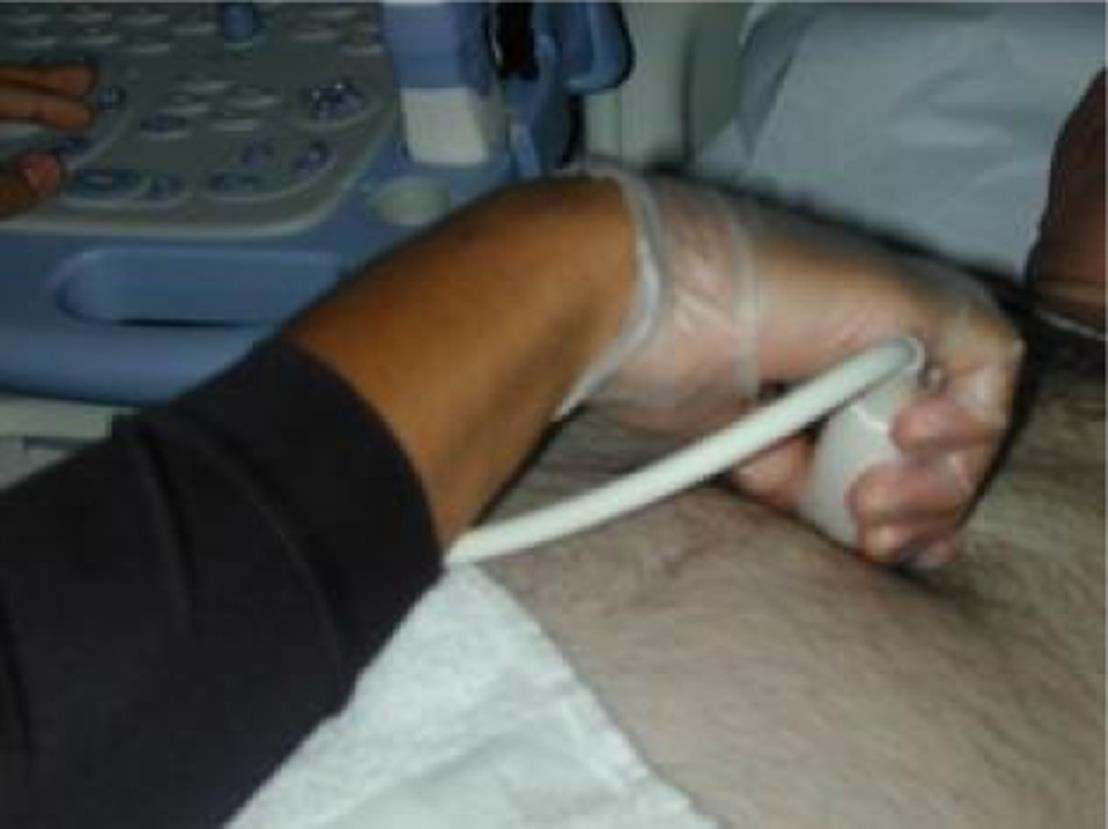
\includegraphics[width=\textwidth]{Figurer/wrist.jpg}
      \caption{Håndledsbøjning og greb om proben \cite{31}}
    \label{wrist}
  \end{minipage}
  \hspace{0.02\textwidth}
  \begin{minipage}{0.47\textwidth}
    \centering
      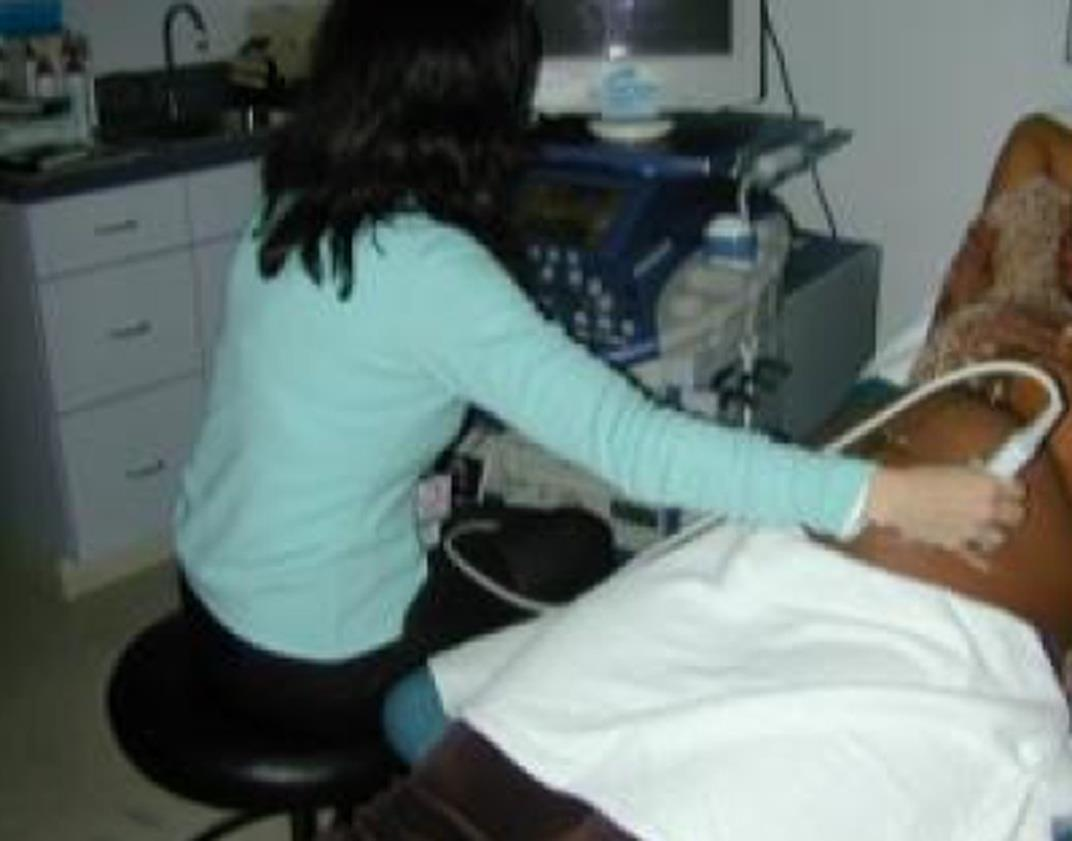
\includegraphics[width=\textwidth]{Figurer/arm.jpg}
      \caption{Arbejde i udstrakt arm \cite{31}}
    \label{udstraktArm}
  \end{minipage}
\end{figure}

Implementeringen af robotarmen vil føre til markante ændringer for sonografernes arbejdsstillinger. Disse ændringer sker idet, sonografen ikke længere skal sidde med udstrakt arm ind over den gravide, og skaderne i skulderen vil derfor kunne undgås. Desuden vil sonografen være mere centreret omkring \textbf{arbejdsstationen - hvilken arbejdsstation?} og derfor vil vrid i kroppen og nakken også blive mindsket. Sonografen skal stadig holde om dummy-proben, se kapitel \ref{Teknologi}, så den gribende belastning kan ikke fjernes helt. Da de resterende belastninger kan mindskes eller helt fjernes, vil dette ikke have den samme belastende virkning. 

En undersøgelse er blevet udført af Robotic Ultrasound for at efterprøve, hvor mange kilo sonograferne skal påtrykke proben med under en ultralydsscanning. Her blev proben påført en dynamometer,hvilken måler trykket sonografen påtrykker med under en scanning. Resultatet heraf blev, at sonograferne ved de almindelige og ukomplicerede scanninger, som en nakkefoldsscanning, trykker med 2-3 kg. Sonograferne skal trykke med omkring 11 kg ved de mere komplicerede scanninger, som scanning på gravide med bagoverbøjet livmoder. Trykket føles dog større for sonografen, da trykket skal påføres i udstrakt arm. Undersøgelsen blev udført på 5 sonografer over én arbejdsdag, se Bilag 12, 28.04.2016.

Den generelle holdning på HEH og RMV er meget teknologivenlig. Derfor formodes det, at implementeringen af teknologien ikke vil føre til væsentlige problemer i forhold til at få sonograferne til at benytte Ultralyds Robotarmen. Implementeringen kræver dog, at der tilrettelægges en ordentlig plan for oplæring af sonograferne i brugen af teknologien. Sonograferne har generelt en god holdning og tillid til teknologi og er åbne for en mulig implementering af Ultralyds Robotarmen.

\subsection{Struktur}
Pr. juni 2016 er den strukturelle opbygning på afdelingerne således, at en medarbejder ultralydsscanner henholdsvis 30 timer på HEH og 22 timer på RMV om ugen. De resterende timer udmønter sig som aflastende arbejde for den enkelte medarbejder. Denne struktur skyldes, at det er et kendt problem på afdelingerne, at scanningsarbejdet er fysisk belastende for medarbejderen. I løbet af en scanningsdag har én medarbejder i gennemsnit ti scanninger. Yderligere foretages der på afdelingerne forebyggende tiltag i form af styrketrænende delastikøvelser, mulighed for gratis massage, ergonomiske redskaber samt fri adgang til fysioterapeuter og wellness-konsulenter, der kontrollerer og vejleder om medarbejderens arbejdsstillinger, se Bilag 4 og Bilag 5.

Afdelingerne tilrettelægger selv mængden af tid den enkelte sonograf skal scanne i løbet af en uge. Dansk Føtalmedicinsk Selskab udstikker hvert femte år anbefalinger, som afdelingerne tilrådes at følge. Anbefalingerne i forhold til antal timers ultralydscanning er 28 timer pr. uge, da det er vurderet, at ved denne mængde af scanninger vil belastningen af sonografen ikke være i en skadende grad, se Bilag 10. Denne vurdering underbygges af videnskabelige forskningsundersøgelser, hvor sonografernes arbejdsskader og mængden af scanningstid er blevet sammenholdt. Disse undersøgelser viser yderligere, at en arbejdsskade typisk optræder efter 5 års arbejde, hvilket der skal tages højde for i valget af observationsgruppe til lignende undersøgelser \cite{35}.

Ud fra dette bemærkes det, at RMV arbejder 6 timer under anbefalingerne, mens sonograferne på HEH scanner to timer mere om ugen end anbefalet. Årsagerne hertil kan være flere. En typisk årsag vil være, at normeringerne og bevillingerne til antal af sonografer og antallet af scanninger, ikke gør det muligt at tilpasse arbejdsforholdet til anbefalingerne. 

Implementering af robotarmen vil føre til en ændring i afdelingernes strukturelle opbygning. Ultralyds Robotarmen vil gøre scanningsarbejdet væsentlig mindre belastende, og dermed vil det kunne føre til, at en medarbejder vil kunne scanne på fuldtidsbasis, altså 37 timer om ugen. Arbejdsstillingerne, som sonograferne udfører, og hvordan disse vil ændre sig, er beskrevet i afsnittet \ref{aktoerer_organisation}. Hvis sonograferne scanner 37 timer om ugen, vil opgaverne de varetager som aflastende arbejde, herunder bl.a. fostervandsprøver, se Bilag 4, og medicinske aborter, se Bilag 5, kunne blive varetaget af andet personale. Yderligere kan det føre til en ændring i antallet af sonografer, der er behov for på den enkelte afdeling. 

HEH har på nuværende tidspunkt indvilliget i at være testafdeling for Robotic Ultrasound ApS under udviklingen og test af produktet. Det er i afdelingens interesse, da der ses en fremtid i produktet. Det ønskes fra afdelingens side at være med under tilpasningen af produktet til afdelingens struktur og behov. 

\section{Delkonklusion}



\chapter{Patient}
Ved implementering af en ny teknologi, herunder en Ultralyds Robotarm, kan det have en indvirkning på patienten. Derfor er det vigtig at belyse, hvilken effekt den nye teknologi har på patientgruppen. \\
I denne MTV vil både gravide og sonografer blive placeret i rollen som patienter. Gravide da de får foretaget en ultralydscanning og sonografer da de ofte oplever arbejdskader. Begge grupper vil derfor blive belyst i dette afsnit.  
\newline
For at kunne udarbejde en fyldestgørende analyse af patientperspektivet er det nødvendigt at belyse flere forhold. Se figur \ref{patientMTV}, hvor de fem patientperspektiver er vist. 
\begin{figure}[h!]\centering
	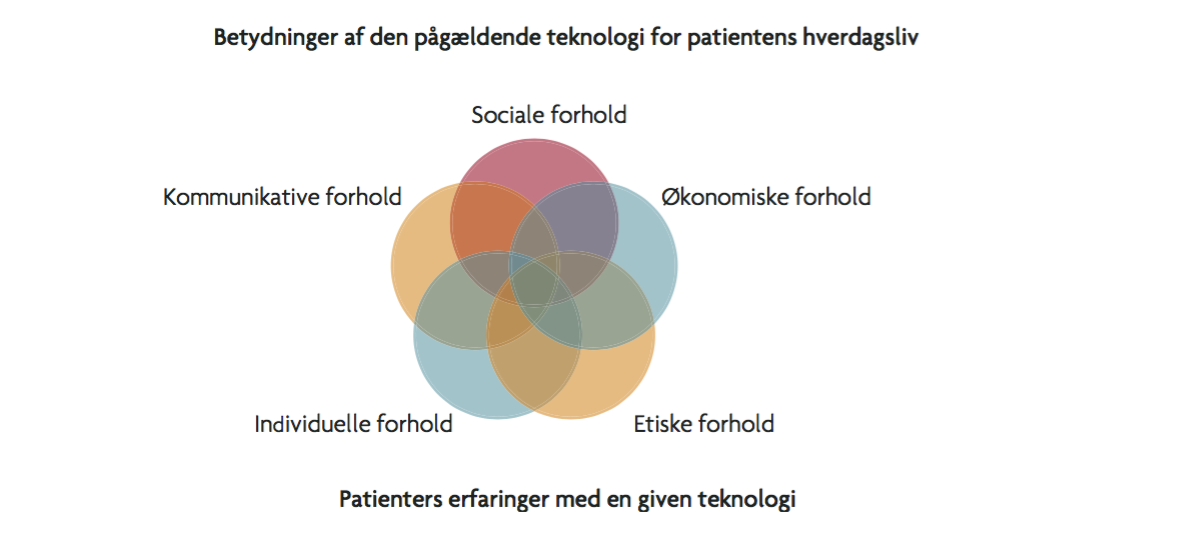
\includegraphics[width = 1.0\textwidth]{Figurer/PatientaspekterMTV}
	\caption{Udforskning af de fem patientaspekter i MTV, som har betydning for patientens hverdagsliv}
	\label{patientMTV}
\end{figure}

\section{Sociale forhold }
\section{Kommunikative forhold}

\section{Individuelle forhold}
\section{Etiske forhold}
Brugen af en Ultralyds Robotarm danner grundlag for en række etiske problemstillinger, som påvirker både gravide og personalet. 
Problemstillingerne omhandler de professionsetiske principper \cite{Husted}: 
\begin{itemize}
	\item \textbf{Pligter}
	\begin{itemize}
		\item Undgå skade af brugeren:\\ 
		Ultralyds Robotarmen skal hverken være til skade for gravide eller personalet. 
	\end{itemize} 
	\item \textbf{Konsekvenser}
	\begin{itemize}
		\item Forebygge sygdom og sygelighed og fremme sundhed eller status quo: \\
		Hvis man ud fra et nytteetisk perspektiv, kan få flere gravide igennem en scanning på kortere tid og samtidig mindske antallet af arbejdsskader for personalet, vil ressourcerne blive udnyttet bedst muligt, og derved komme flest mulige til gavn. Dette følger de socialetiske tanker, som tager hensyn til de mange.    
		\item Lindre lidelse, fremmedgørelse og ubehag:\\
		Ultralyds Robotarmen skal opfylde dette overfor personalet og patienten. Patienten kan føle sig fremstillet som et objekt,  da teknologien kommer tættere på patienten, mens personalet kommer længere væk. Dog er personale til stede i samme rum som patienten, derved er der stadig en form for menneskelig kontakt.  
	\end{itemize}
	\item \textbf{Idealer}
	\begin{itemize}
		\item Handle med forståelse og empati:\\
		Der sker en ændring af nærhed- og omsorgsrelationen mellem den gravide og personalet under en scanning med Ultralyds Robotarmen. 
		\item Handle med etik ansvarlighed overfor personalet:\\
		Ultralyds Robotarmen skal være ansvarlig over for personalet idet at der skal være empati for arbejdssituationen.\\
		Resultatet er at en mindskelse i antallet af arbejdsskader, fremmer personalesikkerhed og -trivsel.   		
	\end{itemize} 
\end{itemize} 

\section{Økonomiske forhold}

\section{Delkonklusion }
\chapter{Teknologi} \label{Teknologi}
I dette afsnit undersøges Ultralyds Robotarmen ud fra et teknologisk perspektiv.  \\
Den teknologiske løsning består af:
\begin{itemize}
\item UR3 Robotarm fra Universal Robots incl. software til styring af denne
\item Stativ til robotten
\item Joystick med dummy-probe
\item Computer
\item Holder til ultralydsprobe
\end{itemize}
Denne løsning skal kobles til det allerede eksisterende udstyr. Derfor er produktet en add-on løsning, hvilket betyder, at produktet skal købes udover det almindelige scanningsudstyr. Det eksisterende system består af Voluson S6 inkl. DICOM (Digital Imaging and Communications in Medicine) og en printer, samt diverse ultralydsprober, se Bilag 4 og Bilag 5.  

%Se bilag økonomi. 
\begin{figure}[H]
	\begin{minipage}{0.45\textwidth}
		\centering
		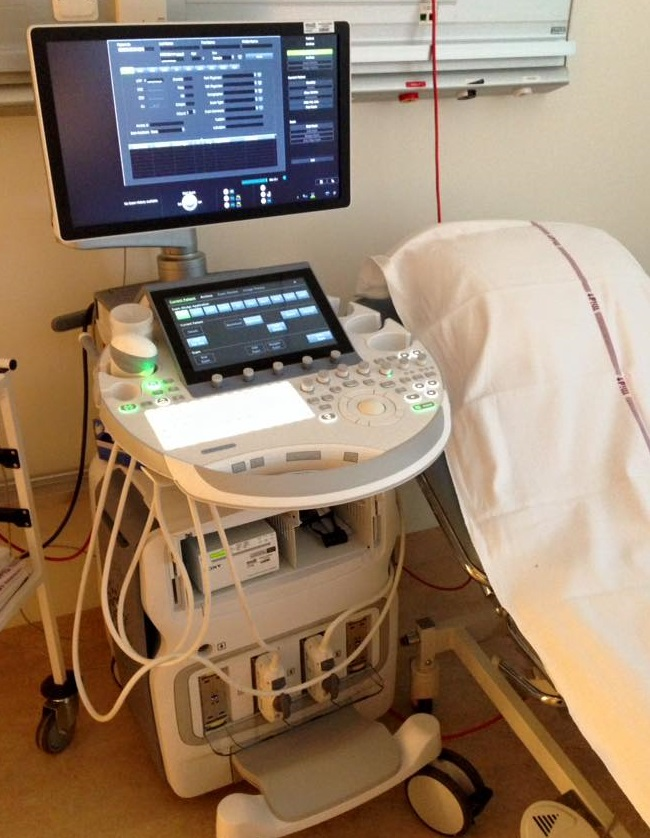
\includegraphics[width=\textwidth]{Figurer/udstyrHorsens.jpg}
		\caption{Nuværende udstyr: Voluson S6 med tilbehør. Billede fra HEH.}
		\label{udstyrHorsens}
	\end{minipage}
	\hspace{0.02\textwidth}
	\begin{minipage}{0.55\textwidth}
		\centering
		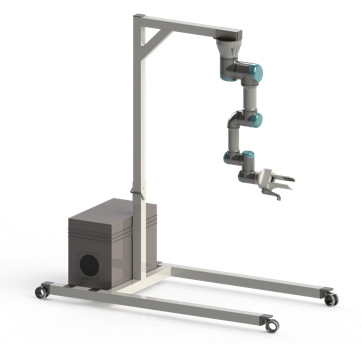
\includegraphics[width=\textwidth]{Figurer/StativMedUR3Render.png}
		\caption{Animation af robotarmen med stativ.}
		\label{Robotstativ}
	\end{minipage}
\end{figure}

\section{Anvendelsesområde}
Produktet skal anvendes til ultralydsscanninger af gravide patienter. Robotarmen er fastmonteret på et stativ, så den kan hænge over den gravide. Dette medvirker til en større trykkraft, end hvis stativet stod på gulvet. For at skabe mobilitet, er stativet placeret på hjul. Hjulene kan låses af sikkerhedsmæssige årsager og for en statisk placering i forhold til den gravide. På robotarmen findes en universalholder til ultralydsproben. Holderen passer til alle større fabrikanters håndholdte ultralydsprober, bortset fra vaginalprober, som robotarmen ikke kan bruges til, se Bilag 12, 28.04.2016.\\

Stativet med robotarmen skal være på den modsatte side af sengen end sonografen. Dette sikrer sonografens udsyn og kontakt til den gravide. \\
Robotarmen holder ultralydsproben over den gravide, mens den styres af sonografen via et joystick. Derved undgår sonografen fysisk akavede arbejdsstillinger.

Joysticket har en dummy-probe, som ikke har nogen probeegenskaber. Den giver sonografen en følelse af at sidde med en ægte probe i hånden.
Systemet skal kunne overføre det tryk, som sonografen påvirker joysticket med til robotarmen, se Bilag 12, 28.04.2016.
 

\begin{figure}[H]\centering
	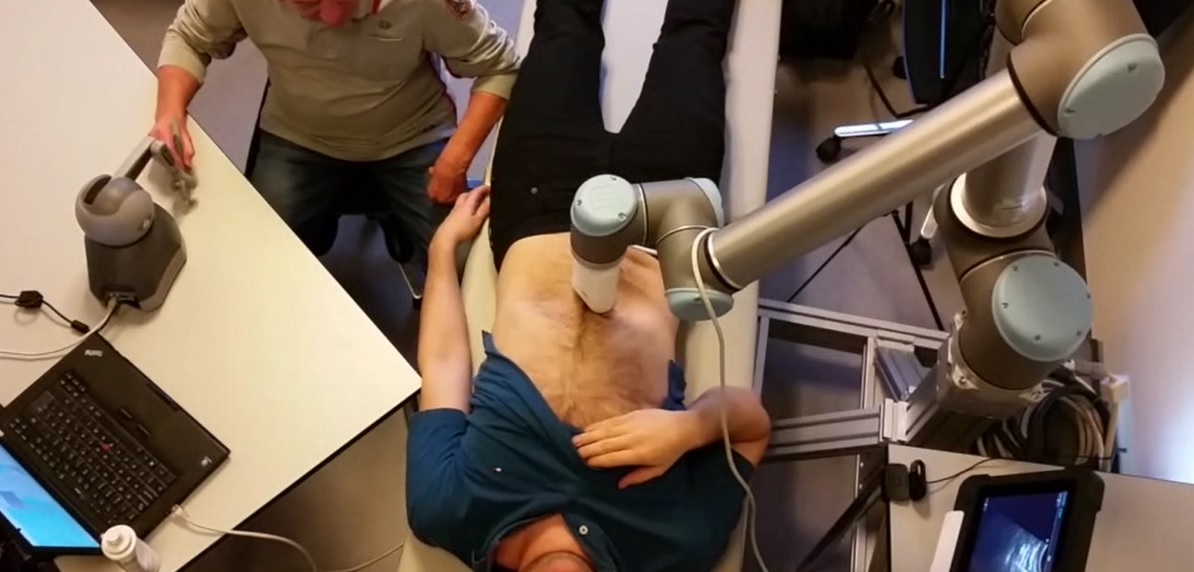
\includegraphics[width = 1.0\textwidth]{Figurer/ergonomiskLosning.jpg}
	\caption{Eksempel på opstilling af Ultralyds Robotarm. Her er robotarmen placeret over patienten og ikke ved side af. På billedet ses joystick(tv.) og robotarm(th.).  }
	\label{ergonomiskLosning}
\end{figure}

\section{Specifikationer}
Robotarmen har en rækkevidde på 50 cm, der angiver hvor langt den kan række ud, som var det en arm. Den vejer 11 kilo, og stativet skal derfor være bygget dertil. Robotarmen har 6-graders frihed, som betyder at den kan bevæge sig i x-, y- og z-aksens retning med drejevirkning om hver akse, se figur \ref{seksgradersfrihed}. Samtidigt kan den lave en +/- 360 graders rotation. \\
Robotarmen kræver en 100-240 VAC, 50-60 Hz strømforsyning, hvilket betyder at den kan blive sat til en almindelig dansk stikkontakt, se Bilag 1.
  
\begin{figure}[H]\centering
	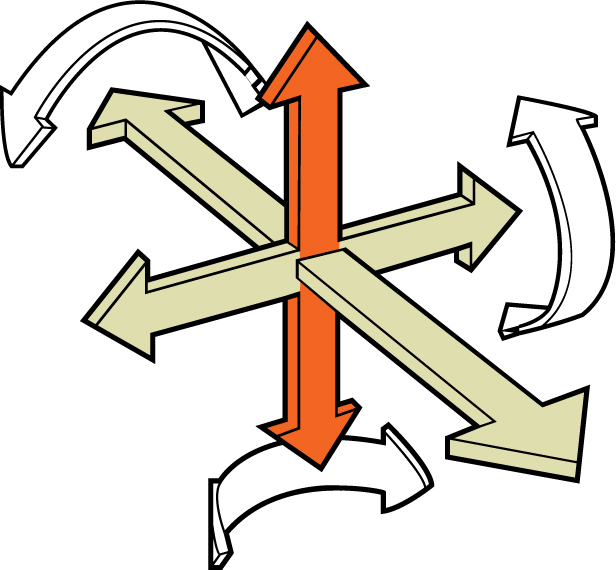
\includegraphics[width = 0.3\textwidth]{Figurer/sixDegressOfFreedom.jpg}
	\caption{Mulige retninger ved 6-graders frihed. Bevægelse i x-, y- og z-aksens retning og drejevirkning om hver akse \cite{6gradersfrihed}. }
	\label{seksgradersfrihed}
\end{figure}

Joysticket har bevægelighed som et håndled, og derved har den også de begrænsninger, som findes ved et håndled. Det har 6-graders frihed, se figur \ref{seksgradersfrihed}, hvilket passer med robotarmen, se Bilag 3. 

Der medfølger software til robotarmen, som er koblingslink mellem joystick og robotarm og styring deraf. Det er her bevægelserne fra joysticket omsættes til robotarmens bevægelser. Her er flere sikkerhedsmæssige foranstaltninger er placeret. Nogle er indbygget i robotarmen - eksempelvis stopper den øjeblikkeligt, hvis den bliver mødt af en kraft på 50 N (ca. 5 kg) eller derover, se Bilag 2.    

\section{Effektivitet}
Det antages at Ultralyds Robotarmen vil blive benyttet til 70-80\% af scanningerne på gravide, da de sidste 20-30\% af scanningerne er for komplicerede til, at robotten kan udføre dem. Derfor skal sonografen manuelt foretage de sidste 20-30\% af scanningerne med den nuværende metode. \\ 
De komplicerede ultralydsscanninger er blandt andet scanninger på kvinder med højt BMI eller kvinder med bagoverbøjet livmoder, se Bilag 12, 28.04.2016. 
 
Ultralyds Robotarmen har ikke indflydelse på billedekvalitet eller kvaliteten af selve scanningen. Dette kommer af, at ultralydsproberne er de samme, som man før har benyttet. \\
Computeren i Voluson S6 indeholder det samme software til billedanalyse og til diverse instrumenter, som bruges under scanninger. Der er blandet andet tale om software til vækst- og flowmålinger af fostre.   \\
Når sonografen vil trykke med ultralydsproben på den gravide, vil trykkraften blive overført til joysticket og dummy-proben, så sonografen får den korrekte trykfeedback. Derved vil sonografen have følelsen af, at der bliver trykket direkte på patienten og kan dermed bedre selv have føling med situationen. \textbf{reference} 

\section{Sikkerhed}
I softwaren til styring af robotarmen findes en sikkerhedsindstilling, hvor en grænse for trykpåvirkningen skal indstilles. Hvis der af menneskelige eller tekniske fejl bliver påvirket med en kraft over grænsen, vil robotarmen automatisk slå fra og stoppe, se Bilag 12, 28.04.2016. \\
Som tidligere nævnt er der også en sikkerhed i, at robotarmen stopper sine bevægelser, hvis den bliver ramt af en kraft på over 50 N, se Bilag 2. Denne foranstaltning gør, at den ikke vil gøre skade på mennesker eller genstande ved at ramme dem, samt at der ikke er behov for et eventuelt sikkerhedsgitter. 

\section{Delkonklusion}
Ultralyds Robotarmen kommer kun til at udføre 70-80\% af scanningerne, hvilket gør at sonograferne stadig skal udføre nogle af scanningerne manuelt. En stor del af belastningen på sonograferne fjernes, når robotarmen kan udfører størstedelen af scanningerne. Sonograferne vil have mere styrke til at udføre de mest komplicerede scanninger manuelt.

Der er tidligere blevet testet med robotarme i forbindelse med ultralydsscanninger, dog på hjertet. Her viste det sig ikke at være et problem at styre selve armen \cite{Hjerterobot}. Denne undersøgelse ligger nogle år tilbage i tiden, og derfor har teknologien allerede ændret sig meget. Det menes ikke at styring, betjening og implementering af Ultralyds Robotarmen til scanninger af gravide vil give de store problemer i sig selv som følge af ny teknologi. Der vil naturligvis altid være en overgangsperiode, hvor sonograferne skal vænne sig til at benytte teknologien. Under perioden vil en scanning muligvis tage længere tid at foretage, for at få den rette kvalitet på resultatet \cite{8}. 
\chapter{Økonomi} \label{Okonomi}
Formålet med dette afsnit er ud fra et økonomisk aspekt at vurdere om en given teknologisk løsning er værd at implementere i praksis. I dette tilfælde gøres det ved at benytte omkostningsminimeringsanalyse. Da det antages, at den sundhedsmæssige effekt er ens i den nuværende situation og i den fremtidige situation, hvor robotarmen implementeres som en add-on løsning til eksisterende ultralydsudstyr. 

Der opstilles to scenarier. Scenarie 1 er den nuværende situation på en ultralydsscannings stue, mens scenarie 2 er den fremtidige situation på en stue med en robotarm. I analysen ønskes det at klarlægge forskellene i de to scenarier, i forhold til hvilke ressource- og omkostningsforhold der er i det enkelte scenarie. Belægget for dette afsnit er skabt pga. interview med ”Kvindeafdelingen, Svangre- og Ultralydsambulatorium” på Hospitalsenheden Horsens (HEH). Her er deres arbejdsgange og arbejdsforhold blevet klarlagt, se Organisation for yderligere beskrivelse heraf. Dermed er det vigtigt at pointere, at forholdene skal være sammenlignelige med HEH førend, at der kan konkluderes tilsvarende for andre afdelinger. 

Yderligere tager analysen udgangspunkt i, at CEO Søren Pallesen hos Robotic Ultrasound forventer, at salgsprisen på robotarmen med tilbehør bliver 400.000 DKK, når den kommer på markedet. Scenarie 2 vil primært bygge på hypoteser, da robotten ikke er færdigudviklet endnu. 

Grundet at robotarmen er en add-on løsning til det eksisterende ultralydsudstyr, er priser på indkøb og vedligehold af ultralydsudstyret ikke medtaget i denne analyse, da det antages at denne må være ens for begge scenarier, og dermed ikke beskriver en forskel. Alle priser i de følgende beregninger er angivet uden moms. 


\section{Scenarie 1 - Den nuværende situation}
I dette scenarie fokuseres der på omkostnings- og ressourceforbruget for at holde en ultralydsscannings stue i drift fem dage om ugen. I den nuværende situation scanner en sonograf fire dage om ugen, mens sonografen den femte dag varetager en række arbejdsopgaver, som sonografen i princippet er overkvalificeret til at varetage. Dette skyldes, at det ønskes at aflaste sonograferne i deres arbejdsforhold, og dermed mindske mængden af arbejdsgener og potentielle arbejdsskader. \\
Omkostningerne i den nuværende situation kan opdeles i følgende punkter. Hver punkt vil blive uddybet og argumenteret senere i afsnittet. 
\begin{itemize}
\item Lønomkostninger
\item Arbejdsgener og -skader
\item Udgifter til forebyggelse
\item Uddannelse af flere sonografer
\end{itemize}
Lønomkostninger er i dette scenarie givet ved 1,2 sonograf. Den 1,2 sonograf er estimeret på baggrund af, at det er nødvendigt, at have en hel sonograf samt 1/5 af en anden sonografs arbejdstid for at have stuen bemandet fem dage om ugen. Månedslønnen for en sonograf med 2 års erfaring med kvalifikationstillæg er på løntrin 6, hvilket giver 26.967 DKK. På årsbasis giver det en årsløn på 323.604 DKK. Lønudgifter er dermed beregnet til:
\begin{equation}
323604 \text{ DKK}\cdot1.2 = 388325 \text{ DKK}
\end{equation}
Det ses også, at i den nuværende organisering af arbejdsgangen er der taget konsekvensen af, at scanning af gravide er et belastende arbejde. Dette viser sig gennem en række omkostninger til forebyggelse af arbejdsskader og -gener. Det koster blandt andet penge, at en sonograf ikke kan scanne fuldtid, og dermed bliver nødsaget til at påtage sig opgaver, sonografen er overkvalificeret til. Disse opgaver vil være billigere omkostningsmæssigt, hvis de bliver varetaget af en person, hvis kvalifikationsniveau passer til opgaven. Denne person vil typisk modtage en lavere løn end sonografen, og dermed vil det føre til en besparelse. 

Samtidig er der udgifter til forebyggelse såsom ergonomiske stole, elastik-træning, massage i arbejdstiden og wellness-konsulenter, der altid står til rådighed, for at give sonograferne råd og vejledning om bedre arbejdsstillinger og -forhold. 

Yderligere er der omkostninger forbundet med uddannelse af sonografer. Uddannelse af en sonograf er estimeret til at koste 108.000 DKK. Uddannelsen foregår som mesterlære over en 16 ugers periode. I denne periode er den nye sonograf altid under vejledning af mesteren. Dermed er der dobbeltbemanding på hver scanning. Således antages det at prisen på uddannelsen er givet ved lønomkostninger til den ekstra mand i form af mesteren i de 16 uger:
\begin{equation}
27000 \text{ DKK}\cdot4 \text{ måneder} = 108000 \text{ DKK}
\end{equation}
Der er dog også forbundet omkostninger med, at sonografen først antages at kunne foretage alle typer scanninger hundrede procent på egen hånd efter to år. Dermed kan der være forlængede scanningstider for den nye sonograf, såfremt vedkommende støder på ukendte ting og bliver nødsaget til at opsøge hjælp fra mere erfarne sonografer. 

Fra et regionsperspektiv er der ikke direkte omkostninger forbundet med, at en sonograf pådrager sig en arbejdsskade grundet dårlige arbejdsforhold. Hvorimod fra et samfundsperspektiv vil det kunne føre til afledte omkostninger, i form af at personen bliver udkørt af arbejdet, og dermed bliver tvunget tidligt på pension. Dermed vil denne person være mindre værd, grundet at denne persons samlede livsløn vil være lavere end en sonograf der har været på arbejdsmarkedet et fuldt arbejdsliv. Dette fører til at denne person koster samfundet penge, fremfor at bidrage til samfundet. 

Hvor stort et problem arbejdsskader er økonomisk, er svært at måle. En arbejdsskade viser sig som en smerte, men det svært at angive smerteværdien i kroner og øre. Yderligere er det svært at svare på om smerten fremkommer af scannings arbejdet eller af en fritidsinteresse sonografen har. Dette gør at arbejdsskader viser sig som afledte omkostninger.

\section{Scenarie 2 - Den fremtidige situation}
I dette scenarie fokuseres der på de ressourcer der vil komme i spil ved implementering af en Ultralyds Robotarm som en add-on løsning til eksisterende ultralydsudstyr. Der tages ligeledes udgangspunkt i omkostnings- og ressourceforbruget for at holde en ultralydsscannings stue i drift fem dage om ugen. I dette afsnit vil der blive trukket paralleller til scenarie 1, for at tydelige gøre hvor omkostnings forskellene er. \\
Omkostningerne i den fremtidige situation er givet ved følgende punkter. Hvert punkt vil blive uddybet i afsnittet.
\begin{itemize}
\item 400.000 DKK til robotarm med tilbehør og stativ
\item Færre arbejdsskader og -gener
\item Ingen udgifter til forebyggelse
\item Regionens ansvar for personale og arbejdsmiljø
\item Lønomkostninger
\end{itemize}
Etableringsomkostninger til robotarmen med tilbehør er estimeret til at være på 400.000 DKK. For de fleste institutioner vil en udgift på 400.000 DKK være et stort udlæg, derfor er det mere relevant at fordele omkostninger over den årrække, som indkøberne afskriver teknologien over. Afskrivnings perioden er på ti år, da det er estimeret at udstyret er forældet efter ti år. Eksisterende ultralydsudstyr afskrives ligeledes over ti år. 

Fordeles etableringsomkostningerne over ti år efter annuitetsmetoden med forrentningsfaktor på 2,2 \%, se Forkortelser og formler, formel 1. Forrentningsfaktoren er estimeres til at være et gennemsnit af inflations renten i Danmark i 2016 og 2020 \cite{inflation}. Årligt giver dette en omkostning på 18.355 DKK:
\begin{equation}
\left(\frac{(1+0.022)^{10}\cdot0.022}{(1+0.022)^{10}-1}\right)\cdot400000 \text{ DKK}=18355 \text{ DKK}
\end{equation}

Det forventes at ved brug af en robotarm ved scanning vil belastningen på sonografen være markant sænket. Det skyldes at sonografen ikke bliver belastet af at påføre store tryk på patienten, samt bevæge arm og skulder ud i dårlige arbejdsstillinger. Dette uddybes i afsnittet Aktører under Organisation \ref{aktoerer_organisation}. Dermed antages i denne analyse, at der i dette scenarie ikke vil opstå arbejdsgener eller -skader grundet scanningsarbejdet. 

Det bevirker at udgifterne til forebyggelse af sonograferne forsvinder. Afdelingen vil dermed ikke have udgifter til ressourcer, som velfærdskonsulenter, ergonomiske stole, aflastende arbejdstider, massage og elastik-træning. I dette punkt adskiller scenarie 1 sig meget fra scenarie 2. Ved besparelse på forebyggelse kan det frigive flere penge til sundhedsfremmende løsninger.

I det første scenarie medførte det i princippet ingen omkostninger for regionen, hvis personalet bliver arbejdsskadet og dermed sygemeldt. Hvorimod det vil være dyrt for samfundet, grundet udbetaling af understøttelse og manglende skatte indkomst. I scenarie 2 er det lige omvendt. Regionen vil have udgiften til robotarmen på 400.000 DKK som en meromkostning, hvilket vil være et stort udlæg hvis der udelukkende ses på tallene. Samtidig har regionen også et ansvar for dens personale og arbejdsmiljø, herunder sikkerhed og sundhed. Dette ansvar gør, at regionen ikke udelukkende fokuserer på tallene, men også vil medtage andre aspekter når en ny teknologi muligvis skal implementeres for at forbedre arbejdsforhold for personalet. 

Samfundet forventer at regionen løfter ansvaret. Således regionen på den måde bidrager til at personalet kan blive i deres arbejdsposition i flere år, og dermed går senere på pension. Et andet aspekt i forhold til regionen er, at regionen ønsker at fremstå godt ud ad til, som en attraktiv region der kan tiltrække arbejdskraft og borgere. 

Det sidste forhold, der er medtaget i denne analyse er forskellene i lønomkostninger. I scenarie 1 skulle der 1,2 sonograf til for at bemande en stue fem dage om ugen. I dette scenarie skal der kun 1 sonograf til. Da det antages, at en sonograf nu kan scanne fem dage om ugen, altså fuldtid, hvorimod sonografen før kun kunne holde til at scanne fire dage om ugen. Dette giver lønomkostninger på årsbasis:
\begin{equation}
323604 \text{ DKK}\cdot1 = 323604 \text{ DKK pr. stue}
\end{equation}
Behovet for færre sonograf til bemanding af én stue, vil sandsynligvis over tid føre til, at færre sonografer skal uddannes. Dette vil føre til en økonomisk gevinst for regionen, da udgifterne til uddannelse af sonografer vil blive nedsat. 

\section{Perspektivering til Regionshospitalet Midt Viborg, Afdeling Kvindesygdomme og Fødsler}
I forbindelse med denne mini-MTV er der også indhentet oplysninger fra RMV gennem et interview. Formålet med interviewet var at få afdækket de samme områder, der blev afdækket ved interview med HEH. 

Set fra et økonomisk perspektiv er omkostningerne til at holde en stue i drift på RMV sammenlignelige med de beskrevne for HEH. Dette viser, at denne omkostnings- og ressourceanalyse er mulig at overføre til lignende afdelinger på andre hospitaler i Danmark. 

\section{Delkonklusion}
Denne gennemgang af omkostnings- og ressourceforskelle mellem scenarie 1 og scenarie 2 viser, at der er en række fordele ved scenarie 1 såvel som scenarie 2. Hvilken der er den afgørende faktor er dermed op til den enkelte potentielle indkøber at afgøre. De største forskelle er ved lønudgifter, penge til forebyggelse og penge til anskaffelse af ultralyds robotarm. 

Hvis der kun kigges på de direkte omkostninger, vil scenarie 1 være den løsning, med mindst omkostninger. Dette skyldes at scenarie 2 er dyrere i direkte omkostninger, da robotarmen er en add-on, og besparelsen på 0,2 sonograf ikke dækker udgiften til robotarmen på 400.000 DKK. \\
Hvis der medtages de indirekte og afledte omkostninger, vil scenarie 2 give mulighed for besparelser for regionen, i forhold til forebyggelse af arbejdsskader og mulige sygedage. Dette kan opveje for udgifterne til robotarmen, men vil naturligvis være afhængig af den enkelte hospitalsafdeling. Scenarie 2 giver mulighed for længere tid på arbejdsmarkedet, hvorved tidlig pension undgås, hvilket giver mindre omkostninger for samfundet.


\chapter{Konklusion}
mindste antallet af akavede stillinger\\
mindre belasting\\
ændring i arbejdsgangen, samme sonograf kan scanne i alle fem dage\\
kun tage 70-80\% af scanningerne \\
Hvor ligger udgifterne henne, de forskellige kasser \\
Ikke den store ændringer for patienten \\
aflaste arbejdsbyrden, mere teknologi i sundhedsvæsenet\\
naturlig udvikling i forhold til at teknologien kommer tættere på \\
ikke medtaget aspekter skal nævnes: de ting som der ses bort fra \\

\chapter{Perspektivering}
I 2007 blev en fremtidig plan fremlagt for landets hospitaler. Her var målet at skære ned på antallet af hospitaler, der har akutmodtagelse døgnet rundt. Antallet skulle gå fra 40 hospitaler i 2007 til 21 hospitaler i 2020. Denne strukturændring skal give færre og mere specialiserede hospitaler, hvilket skal gøre behandlingen bedre og mere effektiv for de danske borgere. Dette betyder, at der bliver en større afstand mellem hospitalerne, da de mindre hospitaler i provinserne lukker \cite{supersygehus}. Dette giver mere transport for borgerne ved rutinemæssige undersøgelser, blandt andet ultralydsscanning af gravide. Her vil Ultralyds Robotarmen fremtidsmæssigt have et potentiale som en telemedicinsk løsning, hvor problemstillingen med store afstande fjernes. Ultralyds Robotarmen vil også kunne afhjælpe situationen i Grønland, hvor der er endnu større afstand mellem borger og hospital \cite{greenland}.

Den telemedicinske udgave af Ultralyds Robotarmen vil imødekomme økonomiske, organisatoriske, samfundsmæssige og patientrelaterede udfordringer. Her vil Ultralyds Robotarmen blive udstyret med kameraer og en mikrofon, som skal transmittere billede og lyd, se Bilag 12, 28.04.2016. Sonografen vil via joysticket kunne scanne den gravide fra afstand. Sonografen behøver derfor ikke at være placeret i samme rum. Ved den gravide skal der være en assistent til stede, som skal klargøre systemet og forberede scanningen.

\begin{figure}[H]\centering
	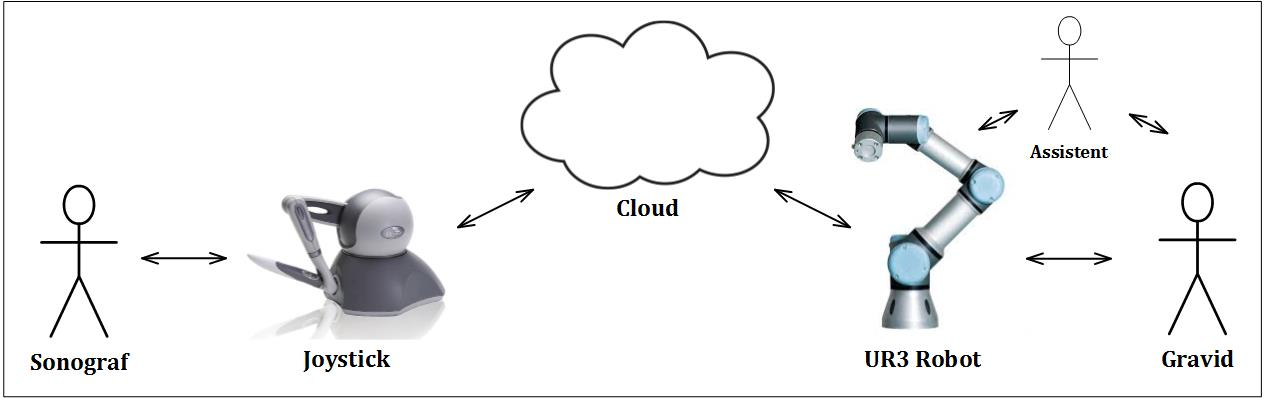
\includegraphics[width = 1.0\textwidth]{Figurer/teknologiTelemedicin.jpg}
	\caption{Sammenhæng mellem systemets dele ved ændring til en telemedicinsk robotarm.}
	\label{systemTelemedicin}
\end{figure}

I Grønland er der få steder, hvor ultralydsscanninger kan udføres og derved store afstande mellem de gravide og sonograferne. Her vil den telemedicinske udgave bevirke, at en sonograf i Danmark, eller et andet sted i Grønland, kan foretage scanningen på gravide placeret afsides steder i Grønland. Dette vil give besparinger på transportudgifter, da patienterne såvel som sonograferne, ikke længere skal transporteres over store afstande ved de rutinemæssige scanninger, se Bilag 12, 18.02.2016. 
Dette vil ligeledes være til gavn i Danmark, hvor ultralydsscanninger vil kunne blive udført i provinserne, selvom sonograferne er placeret i de større byer. Derfor er der potentiale både internationalt og nationalt, da sonografen fra sin egen afdeling vil kunne tilbyde sin ekspertise på tværs af afdelingerne på landets hospitaler. 

Ultralyds Robotarmen som telemedicinsk udgave underbygges af studier, som har undersøgt brugen af ultralyds robotarme som telemedicinske løsninger. Studierne inden for telemedicinsk ultralydsscanning har været i gang i en årrække. Studierne undersøger, hvorvidt det er muligt at få samme kvalitet på telemedicinske scanninger som ved manuelle scanninger. Det undersøges, om billedkvaliteten forbliver den samme, når data skal sendes over internettet. Yderligere undersøges det, om den telemedicinske scanning kan foretages tilfredsstillende \cite{8}\cite{5}\cite{18}\cite{Hjerterobot}. 






\chapter{Referencer}
			%Skal den være der i sidste ende? 

\chapter{Bilag}
\begin{enumerate}
\item Datablad Universal Robots UR3
\item Brochure til Universal Robots UR3
\item Datablad til joystick Geomagic Touch
\item Interview med HEH
\item Interview med RMV
\item Mailkorrespondance med Søren Pallesne
\item Mailkorrespondance med HEH
\item Mailkorrespondance med RMV
\item Mailkorrespondance med Skejby
\item Dansk Føtalmedicinsk Selskab Guidelines
\item Søgeprotokol
\end{enumerate}



\backmatter
\bibliography{bibliografi/Ref}    % Sætter bibliografien bagerst i dokumentet. Bruger bib-filen PRJ3.
\newpage
%\listoffigures	%Figurliste
%\listoftables	%Liste over alle tabeller

\end{document}
